\documentclass[titlepage]{article}

\pagestyle{myheadings}
\markright{\textnormal{17-651 Project 1: Structural Modeling Report - Group 9}}

\usepackage{amsmath,enumerate,zed-csp,graphicx}
\usepackage[margin=1in]{geometry}
\usepackage{listings}
\usepackage{color}
\usepackage{alloy}

\begin{document}
\title{17-651 Models of Software Systems\\[1ex] Project 1: Structural Modeling}
\author{
    {\Large\textbf{Group 9}}\\[3ex]
    Tianli Wu\\[1ex]
    Vishwas Singh\\[1ex]
    Wei-Hsuan Wang\\[1ex]
    Yanhao Li\\[1ex]
    Yuanzong Zhang\\[1ex]
}
\date{\today}
\maketitle
{\bf\Large Task 1}
\begin{enumerate}[\bf\large 1.]
    \item {\bf\large Object model diagram}\\
    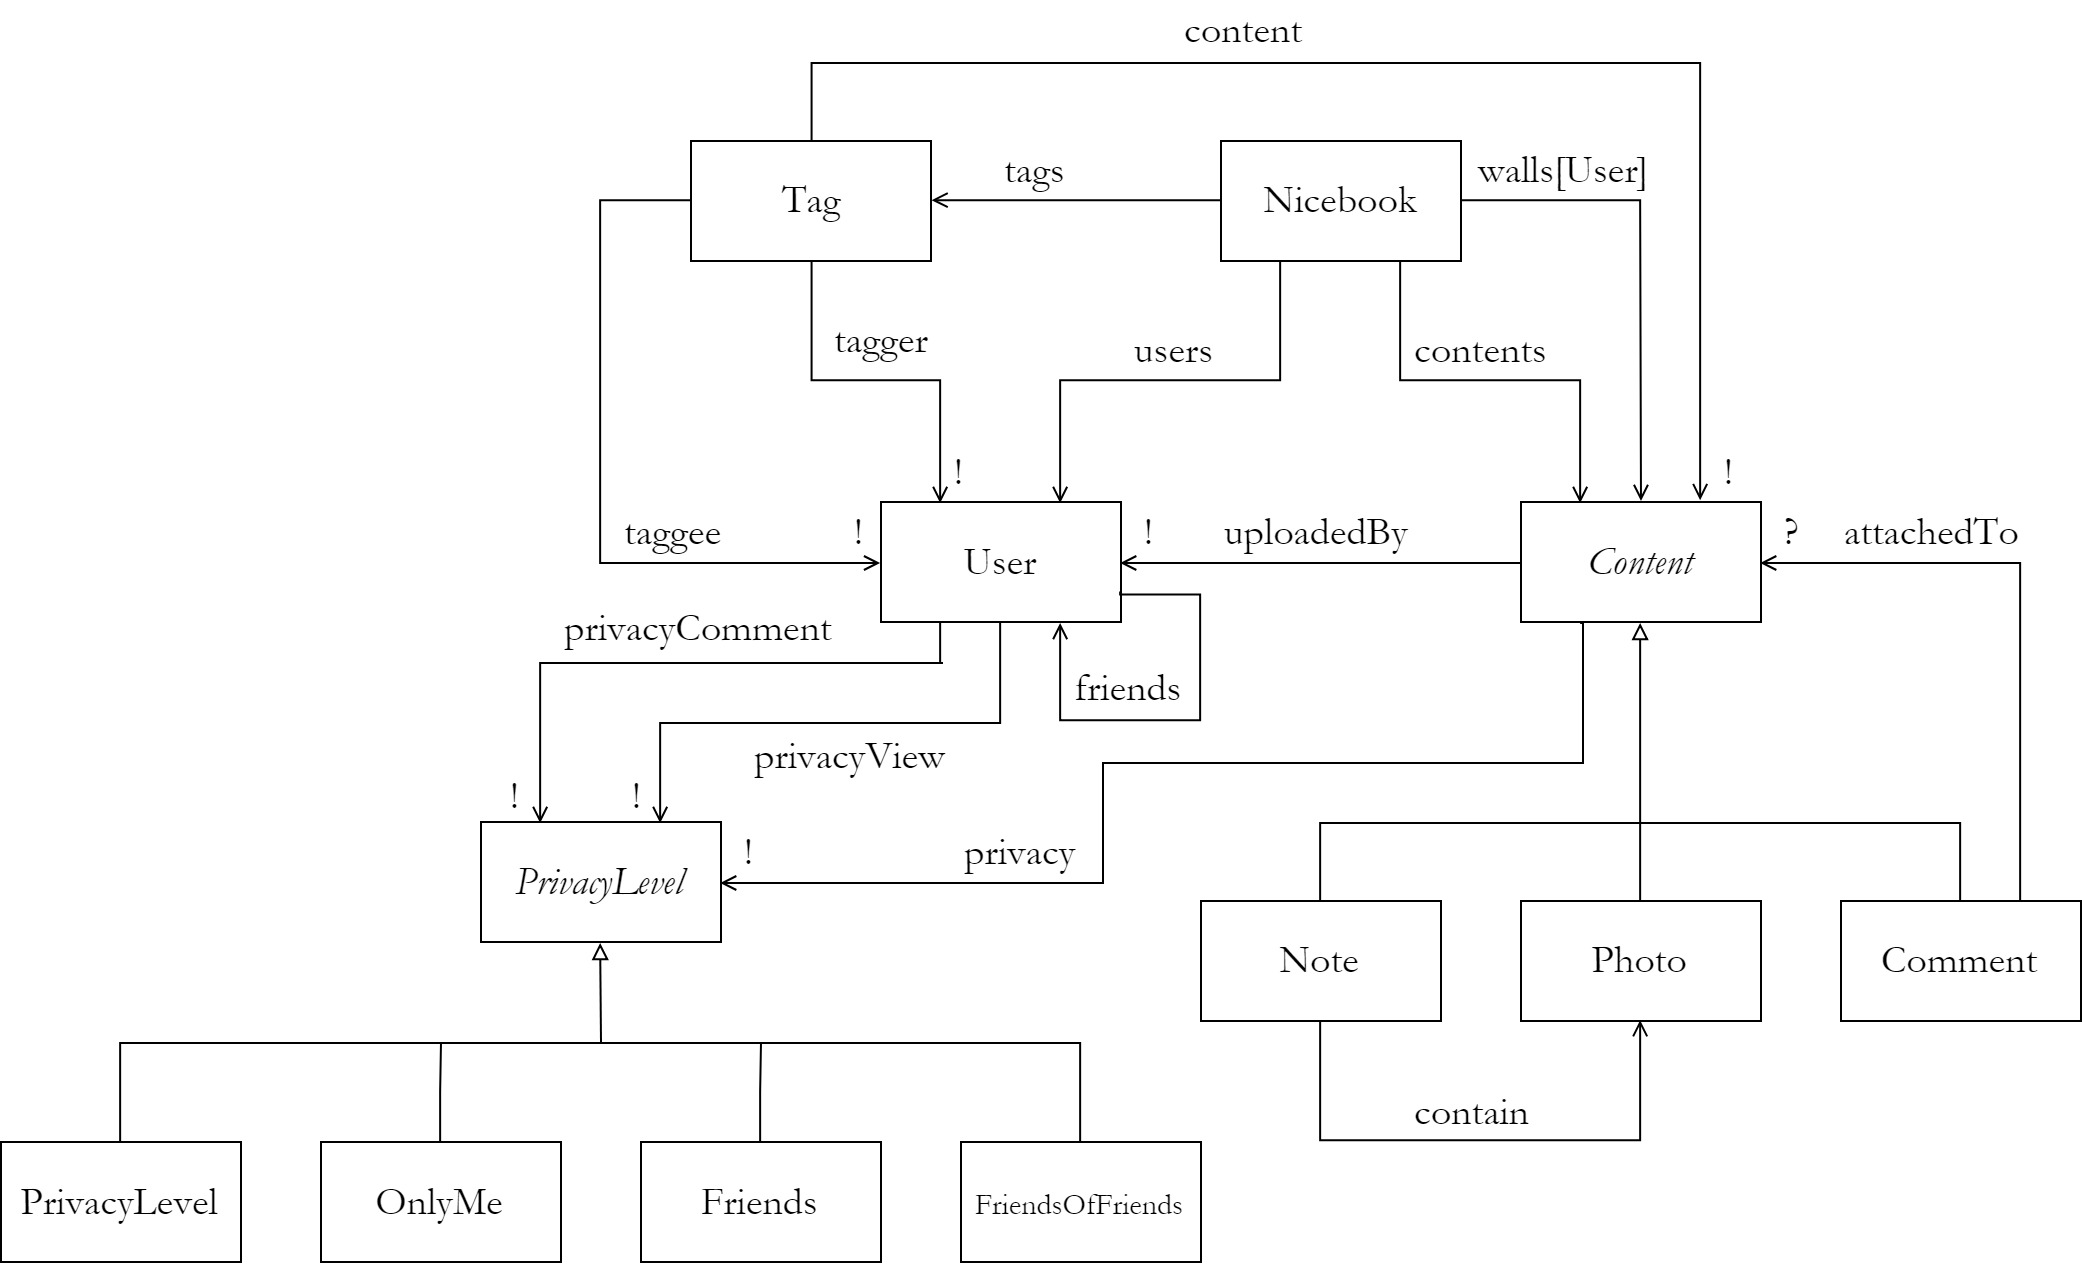
\includegraphics[width=6in]{nicebook.jpg}
    \item {\bf\large Ambiguities and alternatives}\\[1ex]
    Because of the ambiguities of English document, we made several assumptions to ensure our model can account to all possible situations.
    We have considered and rejected several alternative ways to design the system during our modeling process.
    Here, we will first list our assumptions and then talk about the alternatives we have rejected.
    \\[1ex]\textbf{Assumptions: }
    \begin{enumerate}[1)]
        \item A content that has already been uploaded cannot be uploaded again.
        \item A newly-uploaded content has no tag added to and no comment attached to.
        \item The privacy level of a note is the same as the privacy level of all photos it contains.
        \item The uploader of a note is the same as the uploader of all photos it contains.
        \item When a note is uploaded, all the photo(s) it contains is(are) also uploaded.
        \item A newly-uploaded comment cannot be attached to any content.
        \item A content can be removed by its uploader only.
        \item A photo which belongs to a note(some notes) cannot be removed, but it can be removed after the note(s) it belongs has(have) beed removed.
        \item When a content is removed, all the comments and tags associated with that content are removed as well.
        \item When a content is removed, it is unpublished from all the walls of the Nicebook.
        \item A content that has already been published on a user’s wall cannot be published again on the same wall.
        \item The publisher should have permission to view (or directly upload) the content before he/she publishs it.
        \item A user can only unpublish a content from his/her own wall.
        \item A comment always has a privacy level Everyone.
        \item A user must be able to view the content associated with the tag in order to tag other users regarding that content.
        \item A user cannot tag him/herself.
        \item A user cannot tag another user twice to a content. 
        \item The remove tag operation can only be performed by three types of users: the tagger, the user who got tagged, and the owner of the content.
    \end{enumerate}
    \textbf{Alternatives: }
    \begin{enumerate}[1)]
        \item We have considered creating the model without a signature of Nicebook, which means that we consider the entire model as the instance of Nicebook. However, this solution did not work out as we must have a signature of Nicebook to represent the pre-condition and post-condition in Nicebook.
        \item We have considered having a signature called “Wall” to represent each user’s wall. However, if we do this, it will be very hard for us to locate all the walls a specific content has been published on when we try to remove that content. Therefore, we choose to use a User to Content relation to represent the wall.
        \item We have considered representing tag with only a relation. It turned out that it is not enough as it is hard for us to represent the tagger, the taggee, and the content associated with the tag. Hence, we decide to add a “Tag” signature which contains a set of its tagger, a set of its taggee and a set of content associated with it. 
        \item We have considered that a note can contain photos uploaded by other users or with a different privacy level, but it will make the note incomplete when the note is published on some other user's wall.
        \item We have considered that a comment can have a different privacy level. However, sometimes it will make some comments invisible to some users although the users can view the content it is attached to.
        \item We have considered that a user can tag him/herself. However, this action is useless because if he/she hopes to publish the content onto his own wall, he/she can do it directly.
    \end{enumerate}
    \item {\bf\large Implicit assertions}
    \begin{enumerate}[1)]
        \item A content is added a tag to can be published to the taggee's wall only if the content is uploaded by the taggee or his/her friend. Becuase only the wall's owner or his/her friend's content can be published on the wall.
        \item A user can execute an oprtation in Nicebook only if he/she is a user of the Nicebook.
        \item All the contents which are publied on a wall are uploaded to the Nicebook.
        \item All the contents which are attached to by a comment are uploaded to the Nicebook.
        \item All the photos which are contained by a note which has been uploaded to the Nicebook are uploaded to the Nicebook.
    \end{enumerate}
    \item {\bf\large Invariant violation and fixing}\\[1ex]
    When we first check the operation “unpublish”, it violated one of our invariants, which is the content on a user’s wall must be uploaded by the user or his/her friends. The reason for this violation is that we have an imply relation inside predicate “unpublish” like this:
    \begin{alloy}
c in n.walls[u]and c not in Comment implies n'.walls = n.walls - (u -> c)
    \end{alloy}
    In this case, if the content “c” is not on the original wall or “c” is a comment, the entire expression will be true no matter whether we remove the “u->c” relationship or not. Therefore, there might be a situation that the original wall is empty and the wall after “unpublish” contains some contents. The violation is fixed by changing the imply relation to the and relation. Like the following:
    \begin{alloy}
c in n.walls[u]
c not in Comment
n'.walls = n.walls - (u -> c)        
    \end{alloy}
    In this case, the content “c” must be in the original wall and is guaranteed to be unpublished after the operation.
    \item {\bf\large Scopes}\\[1ex]
    We chose $for~12~but~exactly~2~Nicebook$ for all the assertions to check the operations and $runComment$. 
    And we chose $for~12~but~exactly~3~Nicebook$ for $runContent$, $runPublish$ and $runTag$.
    We chose \\$for~15~but~exactly~8~Nicebook$ for $runNicebook$.
    Because for all assertions, we need to check the pre and post condition of the Nicebook, and 2 Nicebooks are enough.
    For $runComment$, we need to prove that the operation is feasible and only one pre and one post conditions are enough.
    For $runContent$, $runPublish$ and $runTag$, we need to prove two operations are feasible so we need two pre and two post conditions. But we can use a post condition of one operaition as the pre condition of another operation.
    For $runNicebook$, we need to prove seven operations are feasible so we need seven pre and seven post conditions. But we can use six post conditions the pre condition of another six operations.
    For other signatures, we try to check as many as possible considering the computing ability of the computer, so we chose the number 12/15 here because with the increment of the scope, the cost of running increases geometrically.\\{}
\end{enumerate}
{\bf\Large Task 2}
\begin{enumerate}[\bf\large 1.]
    \item {\bf\large Function} \texttt{\large viewable}\\[1ex]
    The function is in the alloy file Privacy.sty.
    \item {\bf\large Assertion} \texttt{\large NoPrivacyViolation}\\[1ex]
    The assertion is in the alloy file Privacy.sty.
    \item \texttt{\large NoPrivacyViolation} {\bf\large Satisfication}\\[1ex]
    The violation exists when a content is published to the wall of a user other than the uploader of the content, all the users that follow the privacy level of the wall owner can view the content although they do not follow the privacy level of the content. For instance, according to the diagram, we find that for the Photo2, User2 can view it because it is published on User0’s wall and User0 set his/her privacy level for viewing is Everyone. However, under the privacy setting of Photo2, User2 cannot view it because he/she is neither friend of User1 or friend of a friend of User1.\\[1ex]
    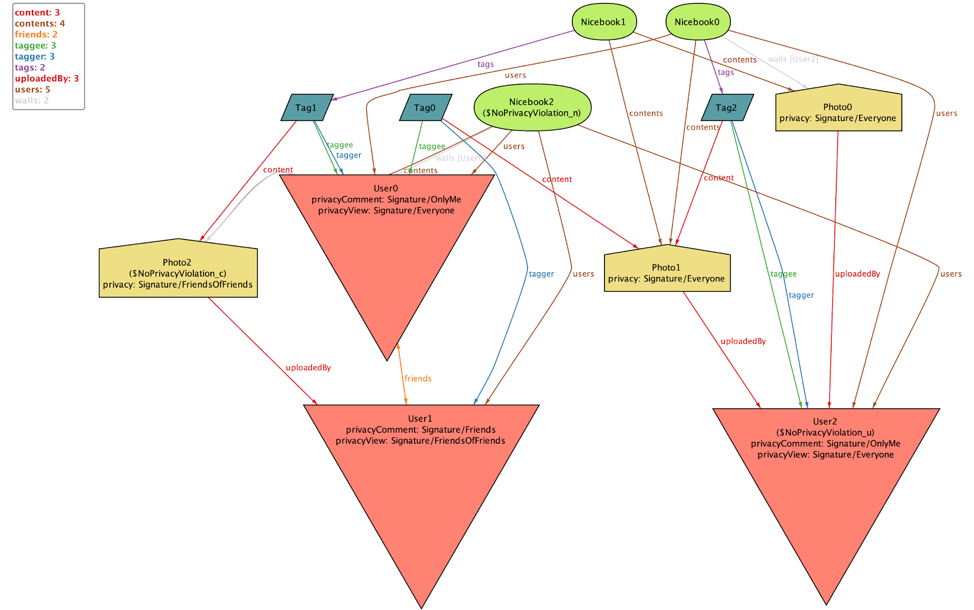
\includegraphics[width=6in]{counterexample.png}\\[1ex]
    The solution we figured out is to take the intersection of the two privacy level. Specifically, a user can view a content only when the content’s owner’s privacy setting and the privacy level of the content itself both allow him/her to see the content. In this case, there won’t be situations that a user who satisfy the privacy setting of the content’s owner while not satisfy the privacy level of the content itself can view the content.\\
    To verify the modification, we changed the predicate contentOnWallCanView and no violation remains.
    \begin{alloy}
// Check whether user u can view content c
// directly on the wall of u'
pred contentOnWallCanView[n : Nicebook, u, u' : User, c : Content] {
    // content c should be on the wall of u'
    c in n.walls[u']
    // follow the privacy level of content c
    privacyFollow[u, c.uploadedBy, c.privacy]
    // if content is not uploaded by u', then follow
    // the view privacy level of u'
    u' != c.uploadedBy implies privacyFollow[u, u', u'.privacyView]
}
    \end{alloy}
\end{enumerate}
{\bf\Large Source Code}\\[1ex]
{\bf\large Signature.als}
\begin{alloy}
// The signature of our social network 
sig Nicebook {
    // set of users in the social network
    users : set User,
    // the unique walls for each user
    walls : users -> Content,
    // set of contents in the social network
    contents : set Content,
    // set of tags
    tags : set Tag
}

sig User {
    // set of friends for a user
    friends : set User,
    // user's privacy setting of who can view his/her content
    privacyView: one PrivacyLevel,
    // user's privacy setting of who can add comment to his/her content
    privacyComment: one PrivacyLevel
}

abstract sig Content {
    // the user that upload this content
    uploadedBy : one User,
    // the privacy level of this content
    privacy : one PrivacyLevel
}

/*
*  	A content must be one of the following three types:
* 	a photo, a note, or a comment
*/

sig Photo extends Content {}

sig Note extends Content {
    // a note may contain one or more photos
    contain : set Photo
}

sig Comment extends Content {
    // a comment can attach to any types of content
    attachedTo: lone Content
}

/*
*  	The signature that represents a tag relation, it contains tagger, 
* 	taggee, and content
*/

sig Tag {
    // the user who perform the tag action
    tagger : one User,
    // the user who got tagged
    taggee : one User,
    // the content that is associated with the tag
    content : one Content
}

/*
* 	Every content must have a privacy level, and the privacy
*	level must be one of the following four types:
*	only me, friends, friends of friends, and everyone
*
*	Each user must have a privacy level as well
*/

abstract sig PrivacyLevel {}
// u : User
one sig OnlyMe extends PrivacyLevel {}
// u.friends + u
one sig Friends extends PrivacyLevel {} 
// u.friends.friends + u.friends (u already in this set)
one sig FriendsOfFriends extends PrivacyLevel {}
// User
one sig Everyone extends PrivacyLevel {}    
\end{alloy}
{\bf\large Invariant.als}
\begin{alloy}
open Signature

pred nicebookInvariant[n : Nicebook] {
    // no user can have wall without being Nicebook's user
    no u : User | u not in n.users and (some c : Content | c = n.walls[u])
    // every content in the wall should exist in the Nicebook
    // and it can not be a comment (comment can not exist without
    // attach to some content)
    all u : n.users | all c : n.walls[u] | c in n.contents
        and c not in Comment and c.uploadedBy in u + u.friends
    // all contents of the Nicebook should follow the invariants of contents
    all c : n.contents | contentInvariant[n, c]
    // all users using the wall should follow the invariants of users
    all u : n.users | userInvariant[n, u]
    // all tags of the Nicebook should follow the invariants of tags
    all t : n.tags | tagInvariant[n, t]
}

pred userInvariant[n : Nicebook, u : User] {
    // friendship is a symmetric relation
    all u' : User | u in u'.friends iff u' in u.friends
    // all user's friend should be user of Nicebook
    all u' : u.friends | u' in n.users
    // a user cannot be his/herself's friend.
    u not in u.friends
}

pred contentInvariant[n : Nicebook, c : Content] {
    // comments have no privacy level and
    // can not be attached to itself recursively
    c in Comment implies 
        (c.privacy = Everyone and 
        c not in c.^attachedTo)
    // photos and notes have privacy level
    else (one p : PrivacyLevel | p = c.privacy)
    // notes should follow its invariants
    c in Note implies 
        (all c' : c.contain | 
            c.privacy = c'.privacy and 
            c.uploadedBy = c'.uploadedBy)
    // content should be uploaded by the user of Nicebook
    c.uploadedBy in n.users
    // content uploaded should follow the user invariant
    userInvariant[n, c.uploadedBy]
}

pred tagInvariant[n : Nicebook, t : Tag] {
    // a user can not tag him/herself
    t.tagger != t.taggee
    // both tagger and taggee must be users in Nicebook
    t.tagger in n.users
    t.taggee in n.users
    // both tagger and taggee should follow the user invariant
    userInvariant[n, t.tagger]
    userInvariant[n, t.taggee]
    // the content associated with the tag must be with the Nicebook 
    //and follow the content invariant
    contentInvariant[n, t.content]
    t.content in n.contents
    // a user can not tag a comment
    t.content not in Comment
}    
\end{alloy}
{\bf\large Privacy.als}
\begin{alloy}
open Signature
open Invariant

// Check whether u has permission to the content/wall of u'
// with a privacy level of p
pred privacyFollow[u, u' : User, p : PrivacyLevel] {
    // everyone
    p = Everyone or 
    // friends of friends
    (p = FriendsOfFriends and u in u' + u'.friends + u'.friends.friends) or
    // friends
    (p = Friends and u in u' + u'.friends) or
    // only me
    (p = OnlyMe and u = u')
}

// Check whether user u can view content c
// directly on the wall of u'
pred contentOnWallCanView[n : Nicebook, u, u' : User, c : Content] {
    // content c should be on the wall of u'
    c in n.walls[u']
    // a user can view all contents on his/her own wall
    u = u' or (
        // if content is uploaded by u', then follow the privacy level of content
        u' = c.uploadedBy implies privacyFollow[u, u', c.privacy]
        // if content is not uploaded by u', then follow
        // the view privacy level of u'
            else privacyFollow[u, u', u'.privacyView]
    )
}

// Find a set of contents on wall that the current content belongs to
fun onWallContent[n : Nicebook, c : Content] : set Content {
    // Find content c' in some user's wall that
    {c' : n.contents | some u : n.users | c' in n.walls[u] and (
        // c is c'
        c' = c or
        // c is a comment and c is attached to c' recursively
        (c in Comment and (c' in c.^attachedTo or 
            // c' is a note and c is attached to a photo c'' recusively
            // and c'' is contained by c'
            (c' in Note and (some c'' : n.contents | 
                c'' in Photo and c'' in c'.contain and c'' in c.^attachedTo)))) or
        // c is a photo and c' is a note containing c
        (c in Photo and c' in Note and c in c'.contain)
    )}
}

// Check whether user u can view content c
pred contentCanView[n : Nicebook, u : User, c : Content] {
    some c' : n.contents | some u' : n.walls.c' | 
        c' in onWallContent[n, c] and contentOnWallCanView[n, u, u', c']
}

fun viewable[n : Nicebook, u : User] : set Content {
    // If content c is uploaded by user u, u can view c
    {c : n.contents | u = c.uploadedBy or contentCanView[n, u, c]}	
}

// the assertion NoPrivacyViolation
assert NoPrivacyViolation {
    all n: Nicebook | all u : n.users | all c : viewable[n, u] |
        nicebookInvariant[n] implies privacyFollow[u, c.uploadedBy, c.privacy]
}
check NoPrivacyViolation 
\end{alloy}
{\bf\large Content.als}
\begin{alloy}
open Signature
open Invariant
open Privacy

// User u uploads content c with privacy level p
// c is before upload, c' is after upload
pred upload[n, n' : Nicebook, u : User, c : Content, p : PrivacyLevel]
{
    // Percondition
    // u is a user of Nicebook n
    u in n.users
    // the content is not already in Nicebook n
    c not in n.contents
    // the content is uploaded by user u
    c.uploadedBy = u
    // no tags initially
    c not in n.tags.content
    // privacy level of content is p
    c.privacy = p
    // If c is a comment, it cannot be attached to any content
    c in Comment implies no c.attachedTo
    // Postcondition
    // users, walls, and tags remain unchanged
    n'.users = n.users
    n'.walls = n.walls
    n'.tags = n.tags
    // the content c is added in n'
    // if c is a note, the photos it contains will be uploaded together
    c in Note implies (n'.contents = n.contents + c + c.contain and 
        (all c' : c.contain | c.privacy = c'.privacy and c'.uploadedBy = u))
        else n'.contents = n.contents + c
    // no comment attached to c initially
    all com : n.contents | 
        com in Comment implies c not in com.attachedTo
}

// User u removes content c
pred remove[n, n' : Nicebook, u : User, c : Content] 
{
    // Precondition
    // u is a user of Nicebook n
    u in n.users
    // the content c is uploaded by user u
    c.uploadedBy = u
    // the content c is in Nicebook n
    c in n.contents
    // comments can not be removed
    c not in Comment
    // if c is a photo and is contained by a note
    // it cannot be removed independly
    not (c in Photo and (some c' : n.contents | c in c'.contain))
    // Postcondition
    // users and tags remain unchanged
    n'.users = n.users
    // remove content c from contents
    n'.contents = n.contents - c - (^attachedTo).c
    all u' : n.users | n'.walls[u'] = n.walls[u'] - c
    n'.tags = n.tags - content.c
}

// Check for upload operation
assert UploadCheck {
    all n, n' : Nicebook, c : Content, u : User, p : PrivacyLevel | 
        (userInvariant[n, u] and contentInvariant[n, c] and nicebookInvariant[n] 
            and upload[n, n', u, c, p]) implies nicebookInvariant[n']
}

// Check for remove operation
assert RemoveCheck {
    all n, n' : Nicebook, c : Content, u : User | 
        (userInvariant[n, u] and contentInvariant[n, c] and nicebookInvariant[n] 
            and remove[n, n', u, c]) implies nicebookInvariant[n']
}

run runContent {
    all n : Nicebook | nicebookInvariant[n]
    some n, n' : Nicebook, c : Content, u : User, p : PrivacyLevel | 
        upload[n, n', u, c, p] and userInvariant[n, u] and contentInvariant[n, c] and 
        nicebookInvariant[n] and nicebookInvariant[n']
    some n, n' : Nicebook, c : Content, u : User | remove[n, n', u, c] and 
        userInvariant[n, u] and contentInvariant[n, c] and 
        nicebookInvariant[n] and nicebookInvariant[n']
} for 12 but exactly 3 Nicebook

check UploadCheck for 12 but exactly 2 Nicebook
check RemoveCheck for 12 but exactly 2 Nicebook
\end{alloy}
{\bf\large Publish.als}
\begin{alloy}
open Signature
open Invariant
open Privacy

/*
*	User u publish content c on the wall of u'
*/
pred publish[n, n' : Nicebook, c : Content, u, u' : User, p : PrivacyLevel] {
    // Precondition
    // both u and u' are users in Nicebook n
    u in n.users
    u' in n.users
    // the content c is not already on the wall 
    c not in n.walls[u']
    // a comment can not be published directly
    c not in Comment
    // the publisher must able to view the content
    contentCanView[n, u, c] or u = c.uploadedBy
    // the content is uploaded by the wall's owner or his/her friend
    c.uploadedBy in u' + u'.friends
    // if c haven't been uplaoded yet, c has no comment or tag
    c not in n.contents implies (
        (no com : n.contents | com in Comment and c in com.^attachedTo) and
        c not in n.tags.content and
        c.privacy = p
    )
    // Postcondition
    // publish the content on the wall
    n'.walls = n.walls + u'->c
    // if content c has not been uploaded before publish, upload it
    n'.contents = n.contents + c
    // users and tags remain unchanged
    n'.users = n.users
    n'.tags = n.tags
}

/*
*	User u publish content c from his/her own wall
*/
pred unpublish[n, n' : Nicebook, c : Content, u : User] {
    // the content c must be on the user's wall
    c in n.walls[u]
    // comment can not be directly unpublished
    c not in Comment
    // unpublish content c from user's wall
    n'.walls = n.walls - (u -> c)
    // users, contents, tags remain unchanged
    n'.users = n.users
    n'.contents = n.contents
    n'.tags = n.tags	
}

// Check for publish operation
assert PublishCheck {
    all n, n' : Nicebook, c : Content, u, u' : User, p : PrivacyLevel | 
        (userInvariant[n, u] and userInvariant[n, u'] and contentInvariant[n, c] and 
            nicebookInvariant[n] and publish[n, n', c, u, u', p]) implies 
                nicebookInvariant[n']
}

// Check for unpublish operation
assert UnpublishCheck {
    all n, n' : Nicebook, c : Content, u : User | 
        (userInvariant[n, u] and contentInvariant[n, c] and nicebookInvariant[n] 
            and unpublish[n, n', c, u]) implies nicebookInvariant[n']
}

run runPublish {
    all n : Nicebook | nicebookInvariant[n]
    some n, n' : Nicebook, c : Content, u, u' : User, p : PrivacyLevel | 
        userInvariant[n, u] and userInvariant[n, u'] and 
            contentInvariant[n, c] and nicebookInvariant[n] and 
            publish[n, n', c, u, u', p] and nicebookInvariant[n']
    some n, n' : Nicebook, c : Content, u : User | 
        userInvariant[n, u] and contentInvariant[n, c] and nicebookInvariant[n] 
            and unpublish[n, n', c, u] and nicebookInvariant[n']
} for 12 but exactly 3 Nicebook

check PublishCheck for 12 but exactly 2 Nicebook
check UnpublishCheck for 12 but exactly 2 Nicebook 
\end{alloy}
{\bf\large Comment.als}
\begin{alloy}
open Signature
open Invariant
open Privacy

/*
*	User u add comment to content c
*/

pred addComment[n, n' : Nicebook, u: User, c : Content, com, com' : Comment] {
    // Precondition
    // u is a user of Nicebook n
    u in n.users
    // c is a content of Nicebook n
    c in n.contents
    // comment is not attached to itself
    com != c
    // new comment is not an existing one
    com' not in n.contents
    // c can be viewd on someone's wall
    some c' : n.contents | u = c.uploadedBy or 
        (some u' : n.walls.c' | c' in onWallContent[n, c] and 
        contentOnWallCanView[n, u, u', c'] and
        privacyFollow[u, u', u'.privacyComment])
    // comment com is not attached to any content
    no com.attachedTo
    // comment com is uploaded by user u
    u = com.uploadedBy
    // comment com has privacy level Everyone
    com.privacy = Everyone
    // no comment attached to the current comment
    all c'' : n.contents | c'' in Comment implies com != c''.attachedTo
    // Postcondition
    // users, walls, and tags remain unchanged
    n'.users = n.users
    n'.walls = n.walls
    n'.tags = n.tags
    // add comment com' to new Nicebook's content list, remove origin com
    n'.contents = n.contents - com + com'
    // except for the content the comment is attached to
    // every attribute remains
    com'.uploadedBy = u
    com'.privacy = Everyone
    com'.attachedTo = c
}

// Check for addcomment operation
assert AddCommentCheck {
    all n, n' : Nicebook, u: User, c : Content, com, com' : Comment | 
        (addComment[n, n', u, c , com, com'] and userInvariant[n, u] and 
        contentInvariant[n, c] and nicebookInvariant[n] and 
        contentInvariant[n, com] and contentInvariant[n, com']) implies 
            nicebookInvariant[n']
}

run runComment {
    all n : Nicebook | nicebookInvariant[n]
    some n, n' : Nicebook, u: User, c : Content, com, com' : Comment | 
        addComment[n, n', u, c , com, com'] and userInvariant[n, u] and 
        contentInvariant[n, c] and nicebookInvariant[n] and nicebookInvariant[n'] and
            contentInvariant[n, com] and contentInvariant[n, com']
} for 12 but exactly 2 Nicebook

check AddCommentCheck for 12 but exactly 2 Nicebook   
\end{alloy}
{\bf\large Tag.als}
\begin{alloy}
open Signature
open Invariant
open Privacy

/*
*	Add a tag. Tagger, taggee, and content associated
*	are all contained in the Tag signature
*/
pred addTag[n, n' : Nicebook, t : Tag] {
    // a comment can not be tagged
    t.content not in Comment
    // u1, u2 are friends (u1 is tagger, u2 is taggee)
    t.taggee in t.tagger.friends
    // u1, u2 are users of Nicebook
    t.taggee in n.users
    t.tagger in n.users
    // a user can not tag him/herself
    t.tagger != t.taggee
    // the content c is in Nicebook n
    t.content in n.contents
    // the content associated must be uploaded by taggee or its friend
    t.content.uploadedBy in t.taggee + t.taggee.friends
    // tagger must able to view the content 
    contentCanView[n, t.tagger, t.content]
    // no duplicate tags
    no t' : n.tags | t = t'
    
    // users and contents remain unchanged
    n'.users = n.users
    n'.contents = n.contents
    // add the tag
    n'.walls = n.walls + t.taggee->t.content
    n'.tags = n.tags + t
}

/*
*	Remove a tag. Tagger, taggee, and content associated
*	are all contained in the Tag signature
*/
pred removeTag[n, n' : Nicebook, t : Tag, u : User]{
    // user has right to remove the tag
    u in t.tagger + t.taggee + t.content.uploadedBy
    // the tag is in Nicebook n
    t in n.tags
    // a user can not tag him/herself
    t.tagger != t.taggee
    // a comment can not be tagged
    t.content not in Comment
    // u1, u2 are users of Nicebook
    t.tagger in n.users 
    t.taggee in n.users
    // the content c is in Nicebook n
    t.content in n.contents
    // users, walls remain unchanged
    n'.users = n.users
    n'.walls = n.walls
    n'.contents = n.contents
    // remove the tag
    n'.tags = n.tags - t
}

// Check for addtag operation
assert AddTagCheck {
    all n, n' : Nicebook, t : Tag | 
        (nicebookInvariant[n] and tagInvariant[n, t] and addTag[n, n', t]) implies 
            nicebookInvariant[n']
} 

// Check for removetag operation
assert RemoveTagCheck {
    all n, n' : Nicebook, t : Tag, u : User | 
        (userInvariant[n, u] and nicebookInvariant[n] and tagInvariant[n, t] and 
            removeTag[n,n', t,u]) implies nicebookInvariant[n']
}

run runTag {
    all n : Nicebook | nicebookInvariant[n]
    some n, n' : Nicebook, t : Tag | 
        nicebookInvariant[n] and tagInvariant[n, t] and 
            addTag[n, n', t] and nicebookInvariant[n']
    some n, n' : Nicebook, t : Tag, u : User | 
        userInvariant[n, u] and nicebookInvariant[n] and tagInvariant[n, t]
            and removeTag[n,n', t,u] and nicebookInvariant[n']
} for 12 but exactly 3 Nicebook

check AddTagCheck for 12 but exactly 2 Nicebook
check RemoveTagCheck for 12 but exactly 2 Nicebook   
\end{alloy}
{\bf\large Main.als}
\begin{alloy}
open Signature
open Invariant
open Privacy
open Content
open Comment
open Publish
open Tag

check UploadCheck for 12 but exactly 2 Nicebook
check RemoveCheck for 12 but exactly 2 Nicebook
check PublishCheck for 12 but exactly 2 Nicebook
check UnpublishCheck for 12 but exactly 2 Nicebook
check AddCommentCheck for 12 but exactly 2 Nicebook
check AddTagCheck for 12 but exactly 2 Nicebook
check RemoveTagCheck for 12 but exactly 2 Nicebook

run runNicebook {
    all n : Nicebook | nicebookInvariant[n]
    some n, n' : Nicebook, c : Content, u : User, p : PrivacyLevel | 
        upload[n, n', u, c, p] and userInvariant[n, u] and contentInvariant[n, c] and 
        nicebookInvariant[n] and nicebookInvariant[n']
    some n, n' : Nicebook, c : Content, u : User | remove[n, n', u, c] and 
        userInvariant[n, u] and contentInvariant[n, c] and 
        nicebookInvariant[n] and nicebookInvariant[n']
    some n, n' : Nicebook, c : Content, u, u' : User, p : PrivacyLevel | 
        userInvariant[n, u] and userInvariant[n, u'] and 
            contentInvariant[n, c] and nicebookInvariant[n] and 
            publish[n, n', c, u, u', p] and nicebookInvariant[n']
    some n, n' : Nicebook, c : Content, u : User | 
        userInvariant[n, u] and contentInvariant[n, c] and nicebookInvariant[n] 
            and unpublish[n, n', c, u] and nicebookInvariant[n']
    some n, n' : Nicebook, u: User, c : Content, com, com' : Comment | 
        addComment[n, n', u, c , com, com'] and userInvariant[n, u] and 
        contentInvariant[n, c] and nicebookInvariant[n] and nicebookInvariant[n'] and
            contentInvariant[n, com] and contentInvariant[n, com']
    some n, n' : Nicebook, t : Tag | 
        nicebookInvariant[n] and tagInvariant[n, t] and 
            addTag[n, n', t] and nicebookInvariant[n']
    some n, n' : Nicebook, t : Tag, u : User | 
        userInvariant[n, u] and nicebookInvariant[n] and tagInvariant[n, t]
            and removeTag[n,n', t,u] and nicebookInvariant[n']
} for 15 but exactly 8 Nicebook
\end{alloy}
\end{document}